\documentclass{article}
\usepackage{amsmath}
\usepackage{mathtools}
\usepackage{amssymb}
\usepackage{graphicx}

\title{Regressão Linear: Implementação e Teoria}
\author{
    Glauco Fleury
}
\date{}

\begin{document}
\maketitle

\section{Introdução à Regressão Linear}
 
Trata-se em suma de um modelo de 'curve fitting': dado
um domínio que apresenta diversas features, isto é,
tem um número $D$ de características (representado
matematicamente por vetores $x \in \mathbb{R}^{D} $), e
uma imagem $y$ a qual se deseja estimar com a função,
o objetivo é encontrar uma curva a qual melhor se encaixe
nos dados já presentes, de modo que seja possível utilizar
a função que a descreve para tentar predizer resultados 
futuros.

A regressão linear assume que a função buscada terá o
seguinte formato: 

\begin{equation}
    \begin{split}
        f(x, \theta) &=  \theta_{0} + \theta_{1}x_{1} + \theta_{2}x_{2}
        + ... + \theta_{D}x_{D} \\ 
        &= \theta \cdot x
    \end{split}
\end{equation}

Isto é, ela assume que a variável a ser prevista pode ser
entendida como a combinação linear das dimensões do vetor de 
input. Do modo como está escrita, a função buscada será 
necessariamete, uma reta (2D), plano (3D), ou qualquer tipo de
hiperplano para mais dimensões. 

\subsection{Ruído e Probabilidade}

Considerando $y = \hat{y} + \epsilon = f(x,\theta) + \epsilon$,
sendo $\epsilon$ o ruído intrínseco à coleta de dados e 
$f(x,\theta) = \hat{y}$ a melhor previsão do modelo acerca do
real resultado, torna-se necessária a abordagem estatística
sobre a modelagem da regressão. Ela toma o seguinte formato:

\begin{equation}
    p(y|x,\theta) \rightarrow y \sim \mathcal{N}(x \cdot \theta, \sigma^{2}) 
\end{equation}

O que basicamente significa que assumimos que a chance de 
$\hat{y}$ "acertar" $y$ é dada por uma distribuição normal,
em que a maior parte das vezes ele acerta, mas pode errar,
porém a estimativa tem chances menores de cometer erros quanto
mais absurdos eles são.

Considerando que o ruído $\epsilon$
advém de uma função de densidade de probabilidade normal,
com média 0 (a maior parte das vezes, $\epsilon = 0$) e
desvio padrão = $\sigma$, podemos escrever que $\epsilon \sim
\mathcal{N}(0, \sigma^{2})$. A variança dessa normal é 
idêntica à outra devido ao fato do ruído ser o fator comum 
de variação em ambos os casos.

\section{Maximum Likelihood Estimation}

Maximum Likelihood Estimation se resume a buscar o vetor de 
parâmetros $\theta_{MLE}$ tal que a curva descrita melhor se 
adeque aos dados, parametrizando-a de modo a encaixá-la nos
pontos do espaço $\mathbb{R}^{D}$. Para isso, é desejável
maximizar a probabilidade de que cada resultado $y$ advenha
de nosso modelo probabilístico (cuja média nós definiremos
com $f(x,\theta) = x^{T}\theta$). Em resumo, buscamos
(para um número $N$ de vetores $x$):

\begin{align}
    \theta_{MLE} &= \underset{\theta}{\arg\max} 
    \prod_{n=1}^{N} p(y_{n}|x_{n}, \theta) \\
    &= \underset{\theta}{\arg\max} \prod_{n=1}^{N}
    \mathcal{N}(y|x \cdot \theta, \sigma^{2}) \\
    &= \underset{\theta}{\arg\min} 
    - \Sigma_{n=1}^{N} \log (\mathcal{N}
    (y|x \cdot \theta, \sigma^{2}))
\end{align}

Sabe-se que $\mathcal{N}(\mu, \sigma^{2}) = 
\frac{1}{\sigma \sqrt{2\pi}} e^{-\frac{1}{2}
(\frac{x - \mu}{\sigma})^{2}}$, e, portanto, é possível
rescreever $\theta_{MLE}$ na forma:

\begin{align}
    \theta_{MLE} &= \underset{\theta}{\arg\min}[ 
    -N\log(\sigma) -\frac{N}{2}\log(2\pi)
    -\frac{1}{2\sigma^{2}}\Sigma_{n=1}^{N}
    (y_{n} - x_{n}^{T}\theta)^{2}] \\
    &= \underset{\theta}{\arg\min} [
    -\frac{1}{2\sigma^{2}}\Sigma_{n=1}^{N}
    (y_{n} - x_{n}^{T}\theta)^{2}]
\end{align}

Para facilitar, vamos escrever o somatório na forma matricial,
e também igualar a equação acima a uma função, de tal forma
que:

\begin{equation}
    \theta_{MLE} = \underset{\theta}{\arg\min} [L(\theta)]
\end{equation}
\begin{equation}
    L(\theta) = -\frac{1}{2\sigma^{2}}
    ||(Y - X\theta)||^{2}
\end{equation}

Onde $X = [x_{1}, x_{2}, ..., x_{n}]^{T}$ e 
$Y = [y_{1}, y_{2}, ..., y_{n}]^{T}$ .

A partir daqui, para achar o nosso parâmetro, fica claro que
o problema se torna a minimazação de uma função quadrada. Como
a Hessiana de $L(\theta)$ é positiva e semi-definida, fica claro
que estamos lidando com um problema de otimização convexa, ou
seja, é possível encontrar uma solução óptima. 

Efetuando $\frac{dL}{d\theta} = 0$ (tal qual ensinam em cálculo I),
encontra-se uma fórmula para a otimização:

\begin{equation}
    \theta_{MLE} = (X^{T}X)^{-1}X^{T}Y
\end{equation}

O problema com essa fórmula está em encontrar a matriz inversa.
O algoritmo atual mais rápido para tal apresenta complexidade
$O(n^{3})$, o que é sub-óptimo, para dizer o mínimo. Como 
alternativa, é possível utilizar um método iterativo que aproxime
nosso tão sonhado vetor de parâmetros. Nesse projeto, escolhi
particularmente o famoso "gradient descent" para estimar os
valores desconhecidos.

\subsection{Expansão Polinomial}

Como eu havia dito no começo, esse modelo de regressão linear
é limitado pela presença de formas lineares (hiperplanos) para
descrever nossas previsões. Observe o seguinte caso, por exemplo:

\begin{figure}[h!]
    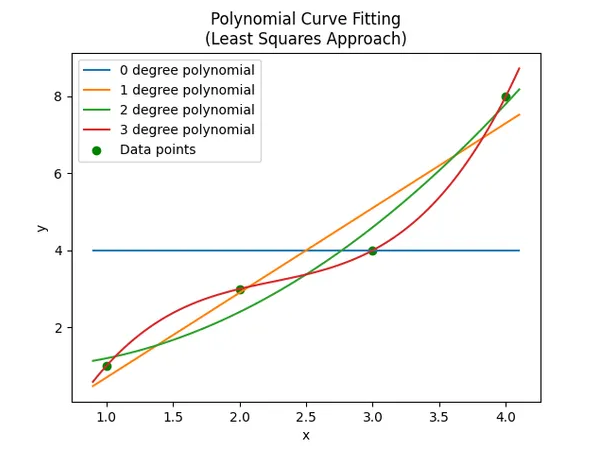
\includegraphics[width=9cm, height=7cm]{pool.png}
    \centering
    \caption{modelagem com diferentes graus de polinômios}
  \end{figure}

Claramente a reta não é adequada para tentar descrever o 
padrão descrito pelos dados. A solução? Expandir polinomialmente
as dimensões analisadas, a fim de capturar padrões mais 
complexos. A isso damos o nome de "polynomial expansion", uma
forma de inclusão de features.

Formalmente, o que buscamos é uma forma de construir um novo
vetor, chamado de feature vector ($\phi(x)$), o qual mudará
o domínio de nossa função para incluir dimensões não lineares.
A função resultante permanece uma combinação linear de dimensões,
já que todos os parâmetros tem grau 1. Desse modo, para
um feature vector qualquer: $\phi(x): \mathbb{R}^{D} \rightarrow
\mathbb{R}^{K}$

O feature vector utilizado nesse projeto é conhecido como
"expansão polinomial": ele expande o vetor $x$ para incluir


\end{document}